\documentclass[10pt,b5paper,oneside]{book}

% **************** PAGE FORMATTING ****************
\usepackage[left=2.5cm,right=2.5cm,top=2.5cm,bottom=3cm]{geometry}
\usepackage[none]{hyphenat}
\sloppy

% ---------------- Fancy Headers ----------------
\usepackage{fancyhdr}

% pagestyle definition: plain
\fancypagestyle{plain}{
	\fancyhf{}
	\fancyhead[L]{}
	\fancyhead[R]{\thepage}
	\renewcommand{\headrulewidth}{0pt}
	\renewcommand{\footrulewidth}{0pt}
}

% pagestyle definition: mmatter
\fancypagestyle{mmatter}{
	\fancyhf{}
	\fancyhead[L]{}
	\fancyhead[R]{\thepage}
	\renewcommand{\headrulewidth}{0.5pt}
	\renewcommand{\footrulewidth}{0pt}
}

\usepackage[utf8]{inputenc}
\usepackage[english]{babel}

% **************** FONT DEFINITIONS ****************
\usepackage{helvet}
\usepackage[T1]{fontenc}
\renewcommand{\familydefault}{\sfdefault}

% **************** OTHER PACKAGES ****************
\usepackage{float}
\usepackage{graphicx}
\graphicspath{{./images/}}
\usepackage[usenames,dvipsnames,svgnames,table]{xcolor}

\usepackage{hyperref}
\urlstyle{same}


% **************** MATH PACKAGES ****************
\usepackage{amsmath}
\usepackage{amsfonts}
\usepackage{amssymb}

\usepackage{amsthm}
\newtheorem{example}{Example}

%% this controls spacing above and below equations
%\setlength{\abovedisplayskip}{3pt}
%\setlength{\belowdisplayskip}{3pt}

\usepackage{circuitikz}
\usepackage{listings}	% code formatting




\begin{document}
\setlength{\parindent}{0pt}
\setlength{\parskip}{6pt}

\frontmatter

\begin{titlepage}

% Frame for the title page
\begin{tikzpicture}[remember picture, overlay]
\draw[line width = 2pt] ($(current page.north west) + (0.5in,-0.5in)$) rectangle ($(current page.south east) + (-0.5in,0.5in)$);
\end{tikzpicture}

% Title page contents
\begin{center}
	\Large eistoolbox \par
\end{center}
\begin{center}
	\large for \par
\end{center}
\begin{center}
	\Large MathWorks\textsuperscript{\textregistered} MATLAB \par
\end{center}

\vspace*{2cm}

\begin{center}
	\large A toolbox for batch fitting Electrochemical Impedance Spectroscopy data to equivalent circuit models
\end{center} 

\vspace*{2cm}

\begin{center}
	\Large User Guide \par
\end{center}
\begin{center}
	\large M.Sc. Juan J. Montero-Rodríguez \par
\end{center}

\vspace*{2cm}

\begin{center}
	\Large Version 0.2-124
\end{center}

\end{titlepage}

\clearpage

\tableofcontents

\mainmatter
\pagestyle{mmatter}

\chapter{Introduction}

\textbf{eistoolbox} is a toolbox for MATLAB\textregistered{} used for batch fitting Electrochemical Impedance Spectroscopy (EIS) data to equivalent circuits models.

In EIS the \textbf{impedance} of a sample is recorded at different frequencies, by applying a small AC voltage signal to the sample, and measuring the current during the experiment. The impedance is stored as a complex number, with the magnitude expressed in Ohms ($\Omega$) and the phase expressed in radians (rad).

As an example, consider the following experiment. An ionic solution of CaCl$_2$ is produced by diluting the salt in water, and stored in a 1 cm$^3$ cubic container. This chamber has two parallel-plate, stainless-steel walls. The impedance is measured from 0.1 Hz to 1 MHz. The experiment is repeated for concentrations of 600, 400, 200, 100, 50, 25, 12, 6, 3, 1.5, 0.8, 0.4, 0.2 mM and then water as reference. In the following magnitude plot, the top turquoise curve is the reference, and the bottom red curve is 600 mM.

\begin{figure}[H]
	\centering
	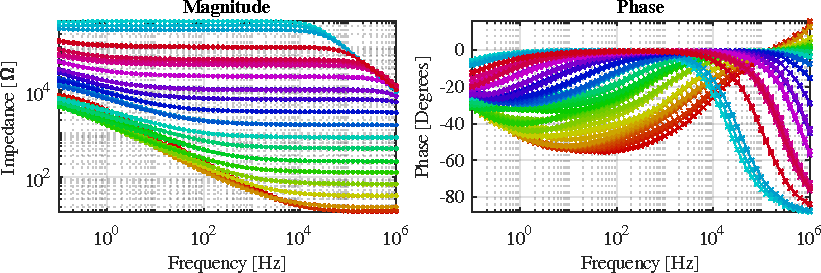
\includegraphics[width=\textwidth]{cacl2}
	\small
	\caption{Impedance spectrum of CaCl$_2$ with different molar concentrations.}
	\label{eiscacl2}
\end{figure}

\clearpage
From the impedance curves of Figure \ref{eiscacl2} one can observe that the ionic concentration affects the impedance and the phase of the sample. For high ionic concentrations, the impedance magnitude is low since abundant ions contribute to the conduction. Low concentration of ions produces a higher impedance since the conductivity is lower.

\section{Circuit modeling}

This impedance is commonly fitted to circuit models, selected depending on the physical characteristics of the measured system. 

For the CaCl$_2$ example, the experimental chamber can be described as a parallel-plate capacitor. The ionic solution has a resistance $R_S$, and the capacitance of the parallel plates is $C_p$. Two additional components have to be included, since the ions in the solution form a double-layer in the proximity of the electrodes. The double-layer is typically modeled by a charge-transfer resistance $R_{ct}$ and a double-layer capacitance $C_{dl}$ which dominate the low-frequency part of the impedance spectrum.

The result of the modeling process is a list of \textbf{circuit elements} such as resistors, capacitors and inductors, and a list of parameter values or \textbf{unknowns}.

The problem is how to calculate these parameters. This is often achieved using \textbf{nonlinear optimization}, and some of the most famous algorithms for fitting EIS data are based on the Complex Nonlinear Least Squares (CNLS) algorithm such as the Levenberg-Marquardt. However there are many algorithms, and they are difficult to implement as they require advanced mathematics.

The present \textbf{eistoolbox} is a collection of algorithms for nonlinear optimization, and a graphical user interface for batch fitting of multiple EIS curves.

\chapter{Theory}


\section{Impedance Spectroscopy}

Electrochemical Impedance Spectroscopy (EIS) measures the complex impedance of a sample as a function of the frequency. An input voltage \eqref{inputvoltage} is applied to the sample, and the current \eqref{inputcurrent} is measured for different frequencies.

\begin{align}
V_i = V \sin(\omega t) \label{inputvoltage} \\
I_i = I \sin(\omega t - \theta) \label{inputcurrent}
\end{align}

The impedance is calculated by means of the Ohm's Law by dividing (\ref{inputvoltage}) by (\ref{inputcurrent})

\begin{align}
Z(\omega) = \dfrac{V_i}{I_i} \\
Z(\omega) = \dfrac{V \sin(\omega t)}{I \sin(\omega t - \theta)} \label{impeqn}
\end{align}

Rewriting (\ref{impeqn}) in complex notation, using polar coordinates

\begin{align}
Z(\omega) = \dfrac{V \angle 0^{\circ}}{I \angle -\theta} = |Z| \angle \theta \label{impcomplex}
\end{align}

Equation (\ref{impcomplex}) describes the impedance of the sample at all possible frequencies. The magnitude of the impedance is dependent of the frequency, since the current is measured independently at each frequency point. The phase is also frequency-dependent.



\section{Dielectric Spectroscopy}

The impedance of the sample, shown in \eqref{impcomplex}, can also be rewritten in rectangular format, by converting the magnitude and phase to real and imaginary parts:

\begin{align}
	R=|Z|\cos{\theta} \\
	X=|Z|\sin{\theta} \\
	Z(\omega) = R + jX \label{impedance}
\end{align}

where R is the resistance and X is the reactance of the sample.

The real part of the impedance is proportional to the resistivity, and the imaginary part is proportional to the permittivity. Both parameters can be calculated directly from the measurements, considering the exact geometry of the electrodes and measurement setup. For parallel plate electrodes, the following equations apply:

\begin{align}
R = \dfrac{\rho L}{A} \label{resistance} \\
C = \dfrac{\epsilon A}{D} \label{capacitance}
\end{align}

The capacitive reactance is given by

\begin{align}
X_C = \dfrac{1}{\omega{}C}	\label{reactivecapacitance}
\end{align}

Substituting \eqref{resistance}, \eqref{capacitance} and \eqref{reactivecapacitance} into \eqref{impedance} results in the following equation \eqref{dielspectr}, which describes the impedance in terms of the resistivity and permittivity of the sample between parallel electrodes:

\begin{align}
Z(\omega) = \dfrac{\rho L}{A} + \dfrac{1}{\omega} \dfrac{D}{\epsilon A} \label{dielspectr}
\end{align}

Impedance Spectroscopy is also referred as Dielectric Spectroscopy, because it gives information about the dielectric properties of the measured sample.

%\newpage
%\section{Kramers-Kronig Transforms}
%
%Experimental data can be validated using the Kramers-Kronig Transforms.
%
%
%\section{Fitting algorithms}
%
%\subsection{Levenberg-Marquardt}
%

\chapter{Quick Start Guide}

Steps for batch fitting impedance data curves:

1. Add files using the "Add file..." button (supported .CSV or .DTA)

Result: A plot of the input files is shown immediately after the files are loaded. Click on the plot buttons to obtain a Nyquist, Bode or Re/Im plot. Save this plot by clicking the save button.

2. Write the circuit string and fitting parameters (or load a .ckt file)

3. Select an algorithm and max iteration number

4. Click the "Fit" button

Result: A plot of the fitted results is shown immediately after the fit process. Click on the plot buttons to obtain a Nyquist, Bode or Re/Im plot. Save this plot by clicking the save button.

5. Save the results using the "Save..." button

\section{Graphical User Interface}

\subsection{Main Window}

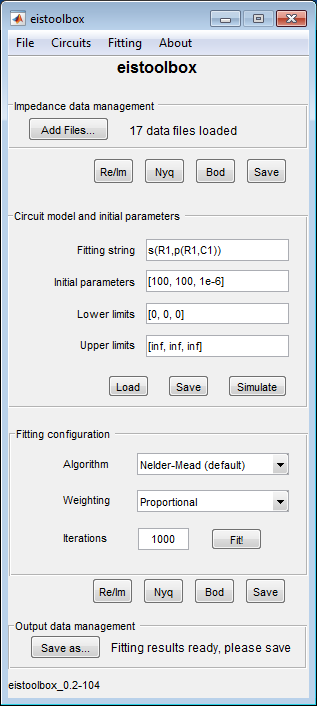
\includegraphics[width=6cm]{main_screenshot.png}

\subsection{Results Window}

The output parameters after the fitting are displayed as a table, in the same order as they appear in the circuit string.

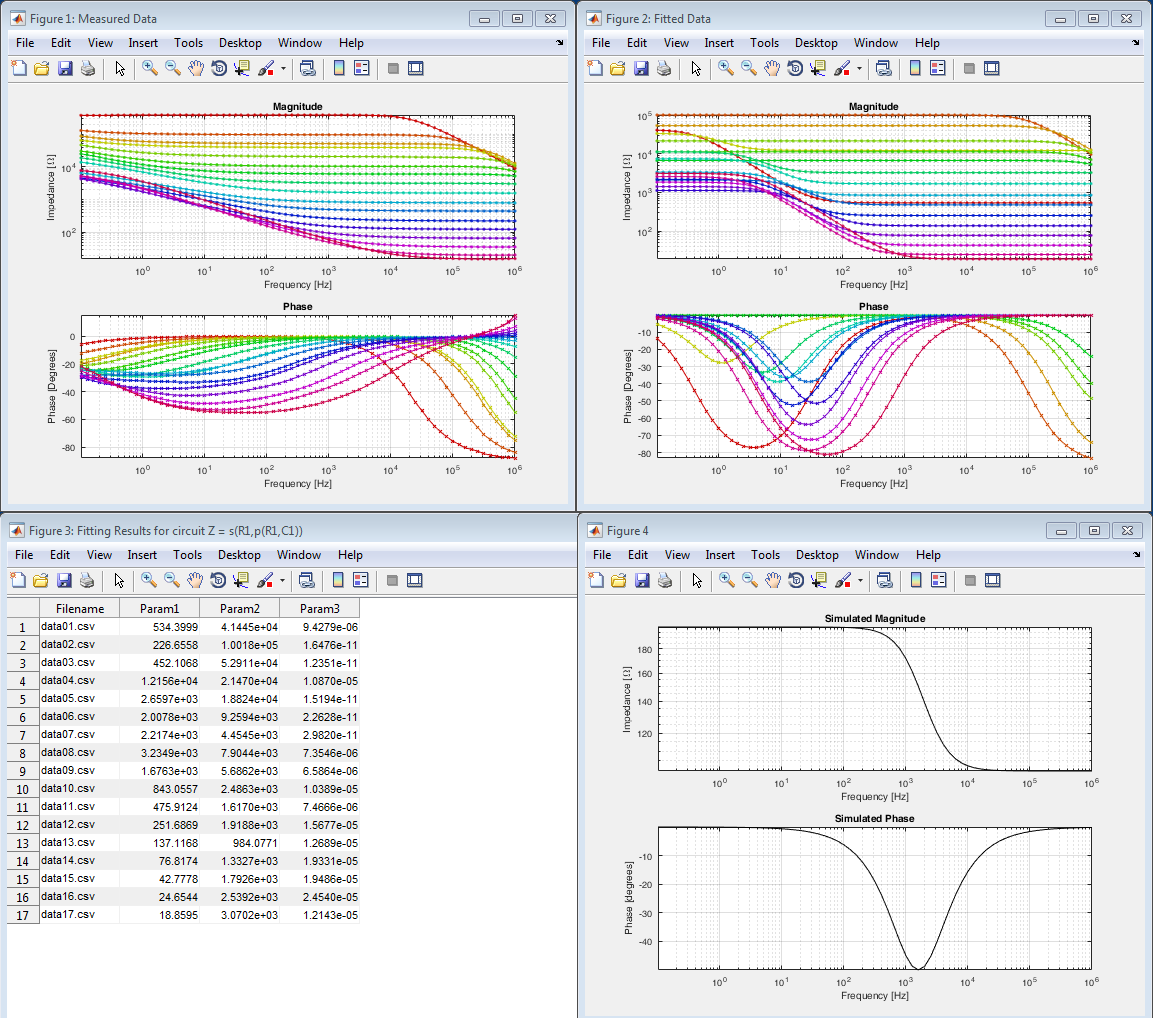
\includegraphics[width=\textwidth]{scr_results.png}

\subsection{Correlations Window}

This window is useful to validate the fitting results. 

There are three correlations implemented: real, imaginary and magnitude. For a perfect fit, the three plots are straight lines where y(x)=x.

Additionally, the fitting results are compared with the original data files by using the Pearson's Chi-square Test of Goodness-of-Fit. This information includes the following parameters: R, chi2, p, fit. These parameters are further explained in Chapter 5.

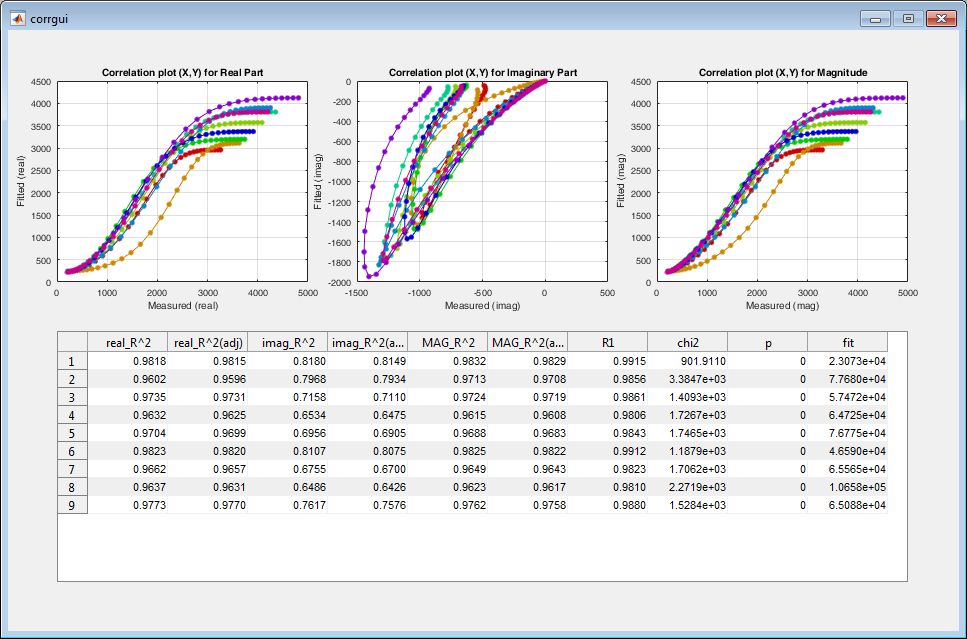
\includegraphics[width=\textwidth]{correlations.png}






\chapter{Equivalent Circuits}

Experimental data is fitted to equivalent circuit models. The models are designed to describe the interfaces, chemical processes and boundaries of the measured setup.

\section{Circuit Elements}

The elements present in the software are described in Table \ref{circelements}:

\begin{table}[h]
	\centering
	\caption{Equivalent circuit elements and their MATLAB implementation.}
	\label{circelements}
	\begin{tabular}{lll}
		\hline \textbf{Symbol} & \textbf{Element} & \textbf{Equation}\\
		\hline R1 & Resistor & $Z(f) = R$ \\ 
		C1 & Capacitor & $Z(f) = 1 / j 2\pi fC$ \\ 
		L1 & Inductor & $Z(f) = j 2\pi fL$ \\
		E2 & Constant Phase Element & $Z(f) = 1 / p_1 (j 2 \pi f)^{p_2} $ \\
		\hline
	\end{tabular}
\end{table}

The Warburg element can be obtained with a Constant-Phase Element by setting $p_2=0.5$


\section{Circuit String Syntax}

Circuits can be built using series and parallel combinations of the elements in Table \ref{circelements}, using the series and parallel operators s() and p(). These operators can contain any number of elements, separated by commas.

The number next to the element letter is the number of free parameters for this element. For a capacitor (C1) the only free parameter is the capacitance. For the constant-phase element (E2) the free parameters are p1 and p2.

\textbf{Common mistake:} Do not write the circuit elements as s(R1,R2,R3,C4...). The elements cannot be written as labels. Instead, write s(R1,R1,R1,C1...).

\section{Circuit Files (.ckt)}

The circuit string, initial parameters and boundary conditions can be stored and loaded from a circuit file with the .ckt extension. This file is read by MATLAB line-to-line. The file should include only four lines with the following content:

Line 1: circuit string

Line 2: initial parameters, sorted in the same order as they appear in the circuit string

Line 3: lower boundary conditions (LB)

Line 4: upper boundary conditions (UB)

Check the folder 'examples\_circuits' for more examples.

\begin{center}
\fbox{ \parbox{\textwidth}{
	\textbf{Example 1: Voigt model in the form R+R//C+R//C+R//C}
	
	\begin{circuitikz}
		\draw 
		(0,0) to[R=$R_S$] (2,0)
		(2,0) to[short] (2,2)
		(2,2) to[C=$C_1$] (4,2) % The resistor
		(4,2) to[short] (4,0)
		(2,0) to[R=$R_1$] (4,0)
		(4,0) to[R=$R_2$] (6,0)
		(6,0) to[R=$R_3$] (8,0)
		(4,2) to[C=$C_2$] (6,2)
		(6,2) to[short] (6,0)
		(6,2) to[C=$C_3$](8,2)
		(8,2) to[short] (8,0)
		(8,0) to[short] (10,0);
	\end{circuitikz}
	
	\vspace{5mm}
	\textbf{Recommended circuit file}
	
	s(R1,p(R1,C1),p(R1,C1),p(R1,C1))
	
	[100,100,1e-6,100,1e-6,100,1e-6]
	
	[0,0,0,0,0,0,0]
	
	[inf,inf,inf,inf,inf,inf,inf]
	
	\vspace{5mm}
	\textbf{Notes}
	
	The elements appear in the circuit string in the following order: RS,R1,C1,R2,C2,R3,C3
	
	The initial parameters, LB and UB have the exact same order
	}
}
\end{center}

\begin{center}
	\fbox{ \parbox{\textwidth}{
			\textbf{Example 2: Ladder circuit in the form: ((((R//C)+R)//C)+R)//C+R}
			
			\begin{circuitikz}
				\draw 
				(6,0) to[R=R3] (8,0)
				(8,0) to[short] (8,2)
				(6,0) to[short] (6,2)
				(6,2) to[C=C3] (8,2)
				(4,2) to[R=R2] (6,2)
				(4,2) to[short] (4,4)
				(4,4) to[C=C2] (6,4)
				(6,4) to[short] (8,4)
				(2,4) to[R=R1] (4,4)
				(2,4) to[short] (2,6)
				(2,6) to[C=C1] (4,6)
				(4,6) to[short] (8,6)
				(0,6) to[R=RS] (2,6)
				(8,6) to[short] (8,0)
				(8,6) to[short] (10,6)
				;
			\end{circuitikz}
			
			\vspace{5mm}
			\textbf{Recommended circuit file}
			
			s(p(s(p(s(p(R1,C1),R1),C1),R1),C1),R1)
			
			[100,1e-6,100,1e-6,100,1e-6,100]
			
			[0,0,0,0,0,0,0]
			
			[inf,inf,inf,inf,inf,inf,inf]
			
			
			\vspace{5mm}
			\textbf{Notes}
			
			The elements appear in the circuit string in the following order: R3,C3,R2,C2,R1,C1,RS
			
			The initial parameters, LB and UB have the exact same order
			
		}
	}
\end{center}


\chapter{Algorithms}

This chapter includes the mathematical description of all the algorithms implemented in the program.

\section{Weighting types}

The fitting algorithms of this toolbox reduce the following distance function (Andrzej Lasia 2014).

\begin{align} \label{distancefun}
dist = S = \sum_{i=1}^{n} \left( w'_i [Z'_i - Z'_{i,calc}]^2 + w''_i [Z''_i - Z''_{i,calc}]^2 \right)
\end{align}

The parameters $w'_i$ and $w''_i$ are the weighting values, computed by one of the following methods:

\begin{tabular}{ll}
	Unit weighting 			& $w'_i = w''_i = 1$ \\
	Modulus weighting 		& $w'_i = w''_i = 1/|Z|^2$ \\
	Proportional weighting 	& $w'_i = 1/(Z')^2$ and $w''_i = 1/(Z'')^2$ \\
	Statistical weighting 	& $w'_i = 1/(\sigma'_i)^2$ and $w''_i = 1/(\sigma''_i)^2$ (not implemented yet)\\
\end{tabular}


\newpage
\section{Minimization algorithms}

\subsection{Nelder-Mead (Simplex)}

The toolbox uses the \textbf{fminsearchbnd} algorithm from John D'Errico.

\subsection{Genetic Algorithm}

ga()

\subsection{Simulated Annealing}

simannealbnd()

\subsection{Constrained Minimization}

fmincon()

\subsection{Other Algorithms}

Not implemented yet

\begin{itemize}
	\item Levenberg-Marquardt
	\item BFGS
	\item Powell
\end{itemize}

\newpage
\section{Statistics}

The overall quality of the fitting can be determined by comparing the original measured data file (expected values) to the simulated values using the fit results (observed values).

Currently the software implements two methods for this comparison: linear regression and Pearson's chi-square test of goodness-of-fit.

\subsection{Linear Regression}

Linear regression is used to compare the original input data with the fitted data.

\begin{itemize}
	\item The real correlation coefficient (rsq\_real) is obtained by linear regression of the fitted vs. measured real part of the impedance. 
	\item The imaginary correlation coefficient (rsq\_imag) is obtained by linear regression of the fitted vs. measured imaginary part of the impedance.
	\item The magnitude correlation coefficient (rsq\_MAG) is obtained by linear regression of the fitted vs. measured magnitude of the impedance.	
\end{itemize}

This is achieved with the following steps:

Linear fit using polyfit
\begin{align}
	p = polyfit(experimental,fitted,1)
\end{align}

evaluate the line to get measured points
\begin{align}
yfitted = polyval(p,experimental)
\end{align}

Residual values
\begin{align}
	y_{resid} = experimental - fitted
\end{align}

square the residuals and get the residual sum of squares
\begin{align}
	SS_{resid} = \sum(y_{resid})^2
\end{align}

compute the total sum of squares by multiplying  variance by n-1
\begin{align}
	SS_{total} = (n-1) * var(experimental)
\end{align}

compute $R^2$
\begin{align}
	R^2 = 1 - \dfrac{SSresid}{SStotal}
\end{align}

compute adjusted $R^2$ to account for degrees of freedom
\begin{align}
	rsq_{adj} = 1 - \dfrac{SSresid}{SStotal} * \dfrac{n-1}{n-p-1}
\end{align}

Where p is the degree of the polynomial used for the regression (in this case p=1: linear)


\subsection{Chi-square Goodness-of-Fit}

The Chi-square parameter is calculated with the following equation (Andrzej Lasia 2014).

\[ \chi^2 = \sum_{i=1}^{n}{\left( \left[ \dfrac{Z'_i - Z'_{i,calc}}{\sigma'_i} \right]^2 + \left[ \dfrac{Z''_i - Z''_{i,calc}}{\sigma''_i} \right]^2 \right)} \]

This parameter depends on the number of points.

Usually it is divided by the number of degrees of freedom $\nu = 2N - m$

\[ \chi^2_v = \dfrac{chi^2}{\nu} = \dfrac{chi^2}{2N - m} \]

N is the number of frequencies: there are 2N measured impedance points (N real and N imaginary)

m is the number of adjustable parameters in the model


%\subsection{Test F}
%
%For comparing two different variances (Lasia 2014)
%
%Not implemented yet.
%
%\[ F = \dfrac{\sigma_1^2}{\sigma_2^2} \]
%
%\subsection{T-test}
%
%For importance of regression parameters (Lasia 2014)
%
%Not implemented yet.
%
%\[ t = p/s_p \]
%
%where $p$ is the value of the parameter and $s_p$ its standard deviation


%\section{Error estimates for individual parameters}
%
%ToDo: This is not yet implemented. It depends on the optimizer functions.


\chapter{Operations menu}

This allows to perform data operations on the RAM memory without modifying the original files. The user can remove any number of points from the end of the files, remove data points higher than a threshold, or plot the data at a specific frequency without fitting.


\section{Remove last N points}

This removes N points from the low-frequency part of the spectrum.

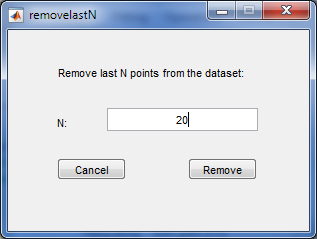
\includegraphics[width=8cm]{remove2.png}

\begin{tabular}{cc}
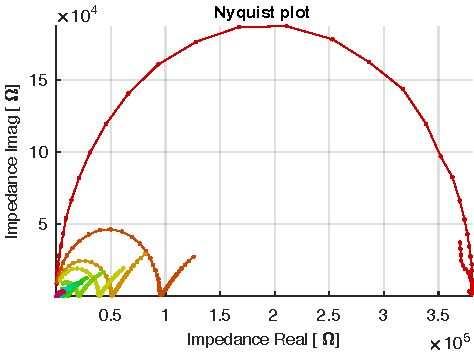
\includegraphics[width=6cm]{remove1.pdf} & 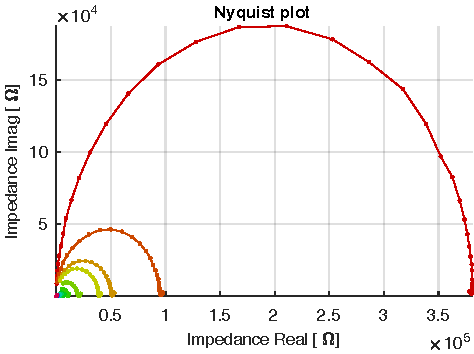
\includegraphics[width=6cm]{remove3.pdf} \\
(a) Original data without modifications. & (b) After removing 20 points. \\
\end{tabular}


\section{Remove values higher than}

This enables to remove points with very high impedance. This can happen when using an Agilent 4284A or similar devices with the GPIB interface, where callibration errors result in high-impedance data points.

The user should be careful not to remove ALL data points accidentally. This can happen if the threshold is too low.

Applying this to the sample files provided:

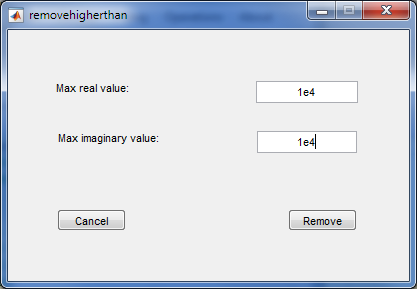
\includegraphics[width=8cm]{hvremove2.png}

\begin{tabular}{cc}
	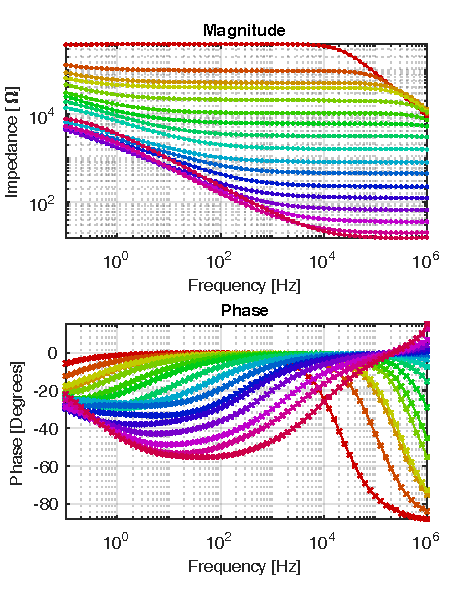
\includegraphics[width=6cm]{hvremove1.pdf} & 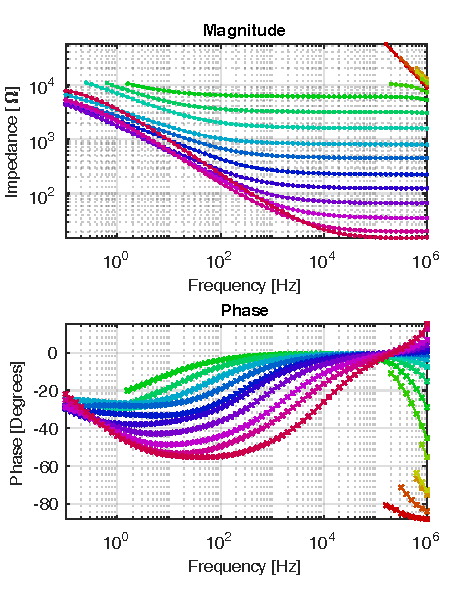
\includegraphics[width=6cm]{hvremove3.pdf} \\
	(a) Original data without modifications. & (b) After removing points $>$ 10e4. \\
\end{tabular}


\section{Plot data at single frequency}

This option plots the data at a single frequency.

The user can input the desired frequency, and data is plotted at the nearest found frequency point.

Notice that if some data was removed earlier, this plots the next closest value.

For the files provided as example, plotting the data at a frequency of 1 MHz:

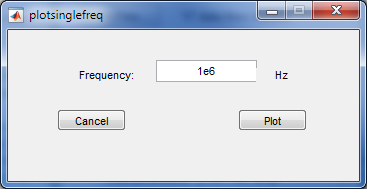
\includegraphics[width=8cm]{plotfreqdialog.png}

\begin{tabular}{cc}
	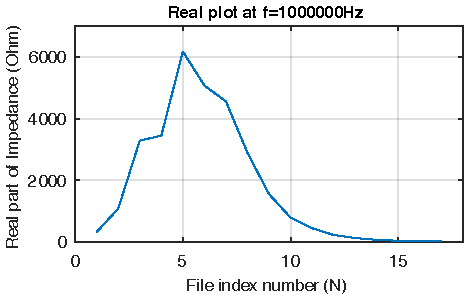
\includegraphics[width=6cm]{plotfreqa.pdf} & 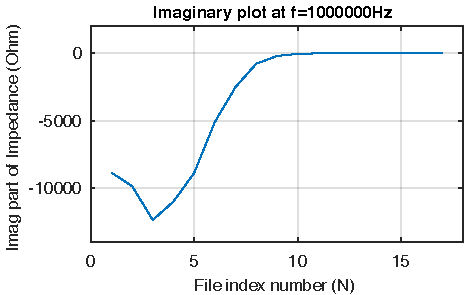
\includegraphics[width=6cm]{plotfreqb.pdf} \\
	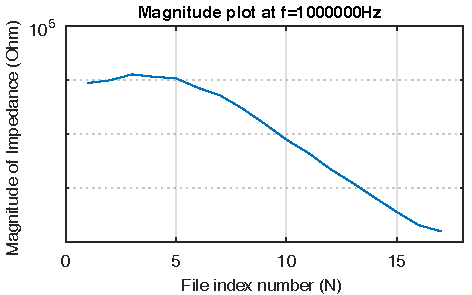
\includegraphics[width=6cm]{plotfreqc.pdf} & 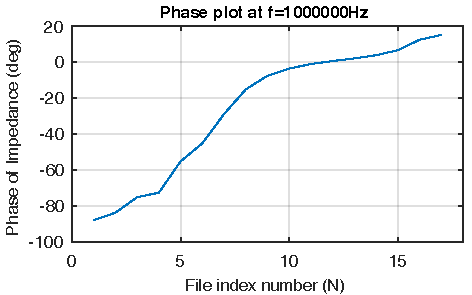
\includegraphics[width=6cm]{plotfreqd.pdf} \\
\end{tabular}

\newpage
\chapter{Licenses for included software}

\section{Zfit}

The original script is available at \cite{Dellis2010}.


\section{fminsearchbnd}

This function was written by John D'Errico and published on MathWorks MATLAB Central under an open-source license. The original file can be downloaded at \cite{DErrico2012}. The function is based on fminsearch and includes the possibility of using boundary conditions, such as the lower and upper limits for the individual circuit parameters.


\section{export\_fig}

This tool is used to save plots as PDF.




% Bibliography

\bibliographystyle{unsrt}
\bibliography{ref}




\end{document}
